\section{System's Perspective}
\label{sec:systems_perspective}

\subsection{Overview}
\label{subsec:systems_perspective_overview}
The initial project was a full stack \textit{Flask} application written in \textit{Bash} and \textit{Python2} with an \textit{SQLite} database. 
This implementation (henceforth referenced as \mini) included refactoring the initial project to the following containerized microservices:
\begin{itemize}
    \item \textit{\cs} backend using the \textit{ASP.NET Core web framework} and \textit{EF Core} object-relational mapping.
    \item \textit{ReactJS} single-page application frontend.
    \item \textit{PostgreSQL} database.
\end{itemize}
Upon which a monitoring stack, and temporarily a logging stack, were added to be served as a containerized application behind a load-balancer on a managed \textit{Kubernetes} cluster (\textit{DOKS})

\subsection{System Design}
\label{subsec:system_design}
% - design of your itu-minitwit systems
The system consists of 5 containerized microservices (see figure \ref{fig:microservices}) of which the largest and most specific to our application is the \cs backend.
It contains all our business logic and provides two open APIs, an Object-Relational Mapping to our database and exposes application-specific PromQL metrics for \textit{Prometheus}. \par

\begin{figure}[h]
    \centering
    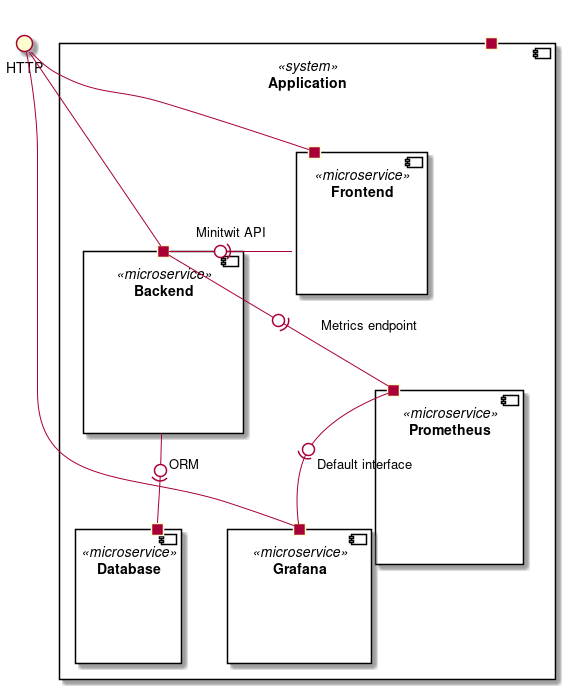
\includegraphics[scale=.5]{images/microservices-components.png}
    \caption{Component diagram of application microservices}
    \label{fig:microservices}
\end{figure}

This design pattern favors load balancing and horizontal scaling as most microservices serve a singular purpose and are non-critical to each-other.
%this will be the module viewpoint

\begin {figure}[H]
    \centering
    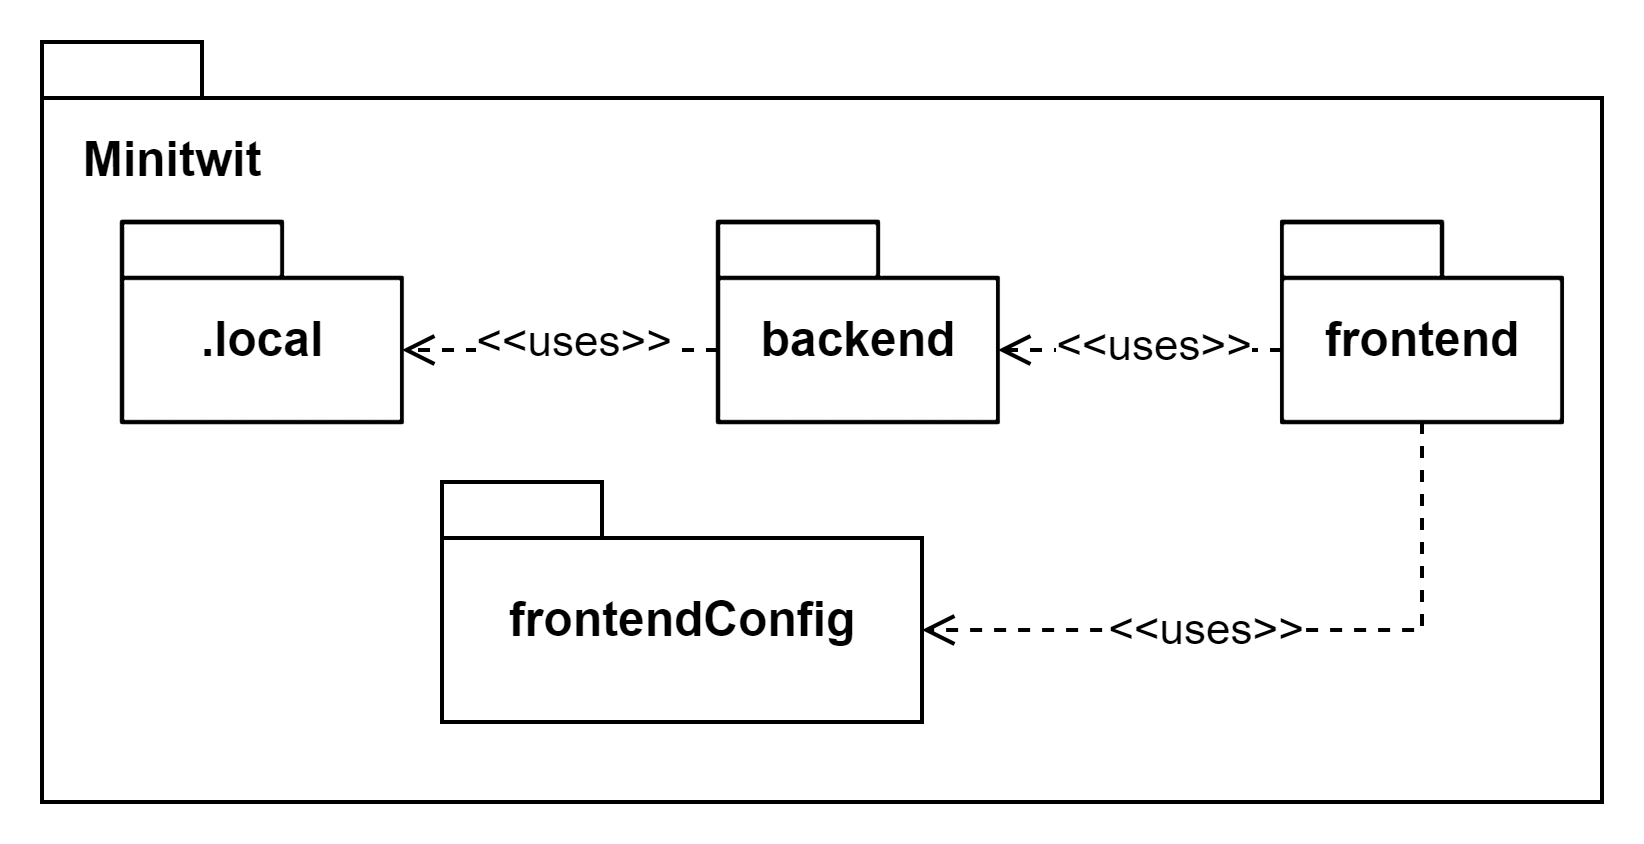
\includegraphics[width=14cm, keepaspectratio]{images/package_class-diagrams/package_diagram.png}
    \caption{Package Overview Diagram From \mini}
    \label{fig:packageOverview}
\end{figure} %should this figure be smaller?
%do we need the .local in this diagram?
The abstract overview of the main packages that makes up the system can be seen in figure \ref{fig:packageOverview}. 
Some files which is in the top main package has been excluded to simply the diagram. 
These excluded files include \texttt{Docker Compose} files, setup files for NGINX and Filebeat etc.
\texttt{frontendconfig} contains some configurations for the \texttt{frontend}, the \texttt{backend} contains everything needed for the system to work, and the frontend includes our UI elements. \\

The most interesting part of the system of \mini is the backend, which decomposition can be seen in figure \ref{fig:decompositionBackend}. 
Some files has been excluded as well in this diagram to simplify it. 
These files include Dockerfiles, Appsettings files, the program.cs file which is the entry point of the system as well as a legacy controller and its interface for the frontend, which is now only used in tests. 
The old controller has been updated by separating it into smaller controllers.

\begin {figure}[H]
    \centering
    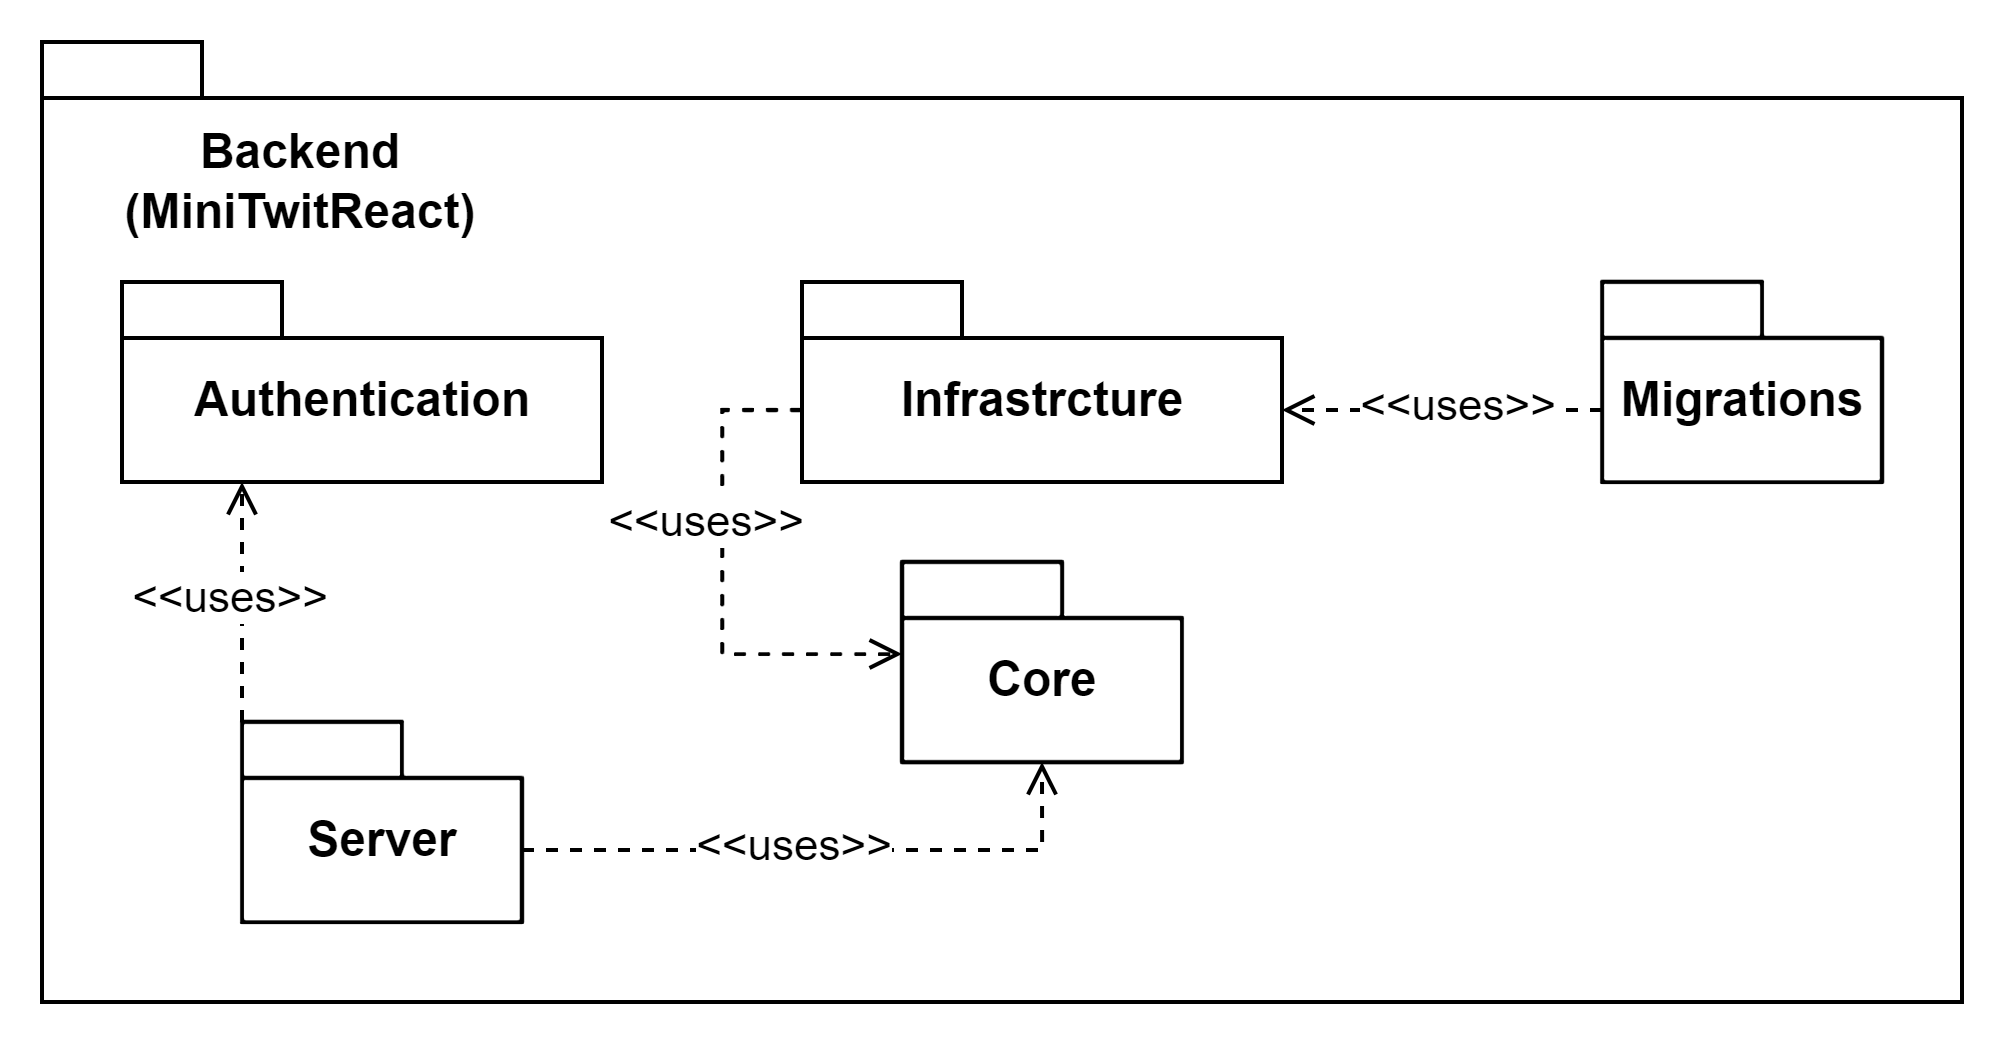
\includegraphics[width=14cm, keepaspectratio]{images/package_class-diagrams/decomposition_backend.png}
    \caption{Decomposition of Backend Package of the \mini System}
    \label{fig:decompositionBackend}
\end{figure}



\subsection{System Architecture}
\label{subsec:system_architecture}
% - architecture of your itu-minitwit systems
% - all dependencies of your itu-minitwit systems on all levels of abstraction and development stages.
% - that is, list and briefly describe all technologies and tools you applied and depend on.
The implementation of \mini follows the \textit{Microservice Architecture Pattern}. This is achieved by separating the application into smaller, independently deployable parts. In \hyperref[fig:figdeployworker]{figure 5} it is illustrated how the backend, frontend, database, and monitoring stack are separated and run independently within individual containers. 
They communicate through the nodes' internal network and receive requests through the ingress controller proxy, which encrypts requests using an auto-renewed SSL certificate. 
Secrets are retrieved by individual services from key-value storage, while persistent volumes are claimed through a persistent volume claim. 
See the pod containing the Postgres database in figure 6.

\begin {figure}[H]
    \centering
    \includegraphics[scale=0.45]{images/deployment_diagrams/devopsdiagrams-deployment worker nodes.drawio(3).png}
    \caption{\mini deployment diagram decomposition of worker nodes.}
    \label{fig:figdeployworker}
\end{figure}
The benefits of using microservices include updating and deploying individual services instead of having to bring the entire system down for an update and the option to integrate different stacks and programming languages without issue, e.g., frontend, backend, and monitoring stack. 
Services can also be scaled independently to support the increased load.\\
Microservices do, however, not come without challenges. 
Management and deployment complexity increases heavily when having to deploy services individually. 
That is where DevOps enters the picture. 
"Microservices both enable, and require, DevOps" according to IBM. 
The reason being that adopting the microservices approach would be unmanageable without implementing DevOps practices like automated ci/cd and monitoring\footnote{ibm\cite{microservices}}.\\
The system still needs to support scaling and load balancing, which is achieved by deploying services to a Kubernetes cluster running on \href{https://www.digitalocean.com/}{digitalocean}. 
Further information on the migration to Kubernetes will be provided in \ref{subsec:scaling} scaling and load balancing \\
%before - broken ref \hyperref[subsubsec:scalingprod]{2.7. scaling and load balancing}.
Kubernetes is used for container orchestration to automate service discovery, networking, load balancing, rolling updates, and service health checking. \hyperref[fig:figdeploy]{figure 6} provides a deployment diagram visualizing the deployment of the \mini service on the Kubernetes cluster managed by the digital ocean and shows the worker nodes from \hyperref[fig:figdeployworker]{figure 5} interact with the rest of the cluster.
\begin {figure}[H]
    \centering
    \includegraphics[scale=0.45]{images/deployment_diagrams/devopsdiagrams-deployment k8s.drawio(1).png}
    \caption{\mini deployment diagram}
    \label{fig:figdeploy}
\end{figure}
Through the Kubernetes command-line tool, kubectl, services can be deployed, updated, scaled, and inspected. The load balancer automatically distributes client requests to the proxies of different worker nodes.

\subsection{Technologies \& Tools}
\label{subsec:techs}
\mini depends on a number of different technologies and tools. This section will briefly describe these dependencies.\\

\begin{enumerate}
    \item \textbf{Docker}
    \item \textbf{Docker-Compose}
    \item \textbf{DockerHub}
    \item \textbf{Markdown}
    \item \textbf{Markup languages}
    \item \textbf{.NET 6} - Used for building the backend. Includes:
    \begin{itemize}
        \item \textbf{C\# 10}
        \item \textbf{ASP.NET Core}
        \item \textbf{NuGet} - The .NET package manager. The application dependency tree include all packages installed and their dependencies.
        \item \textbf{Entity Framework Core}
    \end{itemize}
    \item \textbf{React} - Used for building the frontend. Includes:
    \begin{itemize}
        \item \textbf{JavaScript}
        \item \textbf{WebPack}
        \item \textbf{npm} - The node package manager. The application dependency tree include all packages installed and their dependencies.
    \end{itemize}
    \item \textbf{PostgresQL}
    \item \textbf{Grafana}
    \item \textbf{Prometheus}
    \item \textbf{Nginx}
    
    %VCS and CI/CD
    \item \textbf{GitHub}
    \begin{itemize}
        \item \textbf{Git}
        \item \textbf{GitHub Actions}
        \item \textbf{dependabot}
    \end{itemize}
    
    \item \textbf{Code scanning tools}
    \begin{itemize}
        \item \textbf{sonarcloud}
        \item \textbf{CodeClimate}
        \item \textbf{BetterCodeHub}
        \item \textbf{DeepScan}
        \item \textbf{snyk}
    \end{itemize}
    
    \item \textbf{Terraform}
    \item \textbf{Bash}
    \item \textbf{DigitalOcean}
    \item \textbf{Kubernetes}
    \item \textbf{LetsEncrypt}
\end{enumerate}


\subsection{Subsystem Interactions}
\label{subsec:subsystem_interactions}
% - important interactions of subsystems
A notable downside of the microservice architectural pattern is the unreliability of networking interfaces. 
The key feature of eliminating single points of failure and providing high availability to services makes tracking ip addresses problematic.
Kubernetes solves this with the Service object.
\subsubsection{The Service Object}
Services are ADTS providing stable IP addresses, DNS names and ports via loose coupling to Deployments.
Traffic to microservices is sent to DNS addresses which the internal cluster DNS resolves to IP addresses of the relevant Services.
Services then in turn route the traffic to healthy pods by way of an Endpoint object which stores a dynamic list of healthy Pods matching the service object's labels \cite{k8sbook}.

\subsubsection{The Cluster Network}
Kubernetes abstracts a cluster of hosts to a single platform which behaves in many ways as a decentralized operating system, e.g. by providing a filesystem, dns, network and a means to share memory and computational resources. \par
The Cluster Network operates similarly to a local network on any regular host in such a way that any device or process on the network is discoverable by other entities on the same network. 
Hence, given that a pod knows the IP of another pod on the cluster network, traffic between them is possible, though traffic via Service objects is preferable.
\subsubsection{The Ingress Object}
Ingress is all about accessing multiple web applications through a single Service object \cite{k8sbook}. 
The Service object has several subtypes, two of which provide a one-to-one mapping between an internal Service and a public port.
Ingress is a Kubernetes resource which serves various purposes but most importantly provides a reverse proxy to multiple Service objects.
\subsubsection{The Load-Balancer}
Of the briefly mentione
\begin{table}[h!]
    \centering
    \begin{tabular}{|c|} \hline
         Prometheus \\ \hline
         MinitwitAPI \\ \hline
         LoadBalancer \\ \hline
    \end{tabular}
    \caption{Network interfaces}
    \label{tab:my_label}
\end{table}

\subsection{System state}
\label{subsec:system_state}
% - Describe the current state of your systems, for example using results of static analysis and quality assessment systems.
% Wait until after cleanup when frontend is merged.
To be able to argue about the quality of our code, we have enhanced our \textit{CI} pipeline with static code analysis tools. These analyze and rate \mini per their definition of code quality.

\subsubsection{Code Quality, Technical Debt, \& Maintainability}
According to the \textit{Better Code Hub quality status}\footnote{\hyperref[fig:hubStatus]{Better Code Hub quality status}}, our codebase complies with 9 of 10 measures for quality while failing on code duplication. This is because \mini supports both a simulator API and an API for the frontend. When refactoring infrastructure code for the frontend API, we kept the infrastructure for the simulator resulting in code duplication.\\
\textit{Sonarcloud} suggests that we have a technical debt of 55min, all of which is from the \texttt{Simulation Controller} and its infrastructure class, indicating that the simulation \texttt{controller} and \texttt{repository} requires refactoring. It also located 8 code smells but still gives the main branch a grade of A\footnote{\hyperref[fig:cloudMaintainability]{Sonarcloud Maintainability Scores}}. In contrast \textit{Code Climate}\footnote{\hyperref[app:codeClimate]{Code Climate}} scores the technical debt of the system as 2 weeks and finds 17 code smells. This partly shows the difference in the definition of code quality between different tools. However, it is also caused by Code Climate analyzing the entire repository. At the same time, Sonarcloud analyzes only the backend as seen in the Sonarcloud language distribution stats\footnote{\hyperref[fig:codeClimateLangDis]{Sonarcloud language distribution stats}} compared to the Code Climate language distribution graph\footnote{\hyperref[fig:codeClimateLangDis]{Code Climate language distribution graph}}. The frontend contributing heavily to technical debt was expected. The team did not have much experience with React going into the project, so we prioritized the frontend's required functionality and spent time implementing weekly assignments and improving the backend. The difference in the definition of code quality of these tools is fascinating. \textit{DeepScan}\footnote{\hyperref[app:codeAnalDeep]{DeepScan}} suggests no code quality issues. \\
In conclusion, the technical debt of the frontend hurts the maintainability of the system. The backend has little to no technical debt, and code quality is good except for the simulation controller and simulation repository needing refactoring.

\subsubsection{Vulnerabilities}
2 dedicated security vulnerability scanning tools are used to increase chance of discovering and removing vulnerabilities as fast as possible. Both \textit{snyk}\footnote{\hyperref[app:codeAnalSnyk]{Snyk}} and \textit{dependabot}\footnote{\hyperref[app:codeAnalDependabot]{Dependabot}} finds a vulnerability of high severity stemming from a \textit{npm} dependency, enforcing the fact that it is a known vulnerability. \\
In conclusion, the \mini code base contains two vulnerabilities in the frontend npm modules.




\subsection{License Compatibility}
\label{subsec:license_compatability}
% - Finally, describe briefly, if the license that you have chosen for your project is actually compatible with the licenses of all your direct dependencies.
%this is only a draft
The initial license chosen was \textit{MIT}, which means everyone can use and modify the code freely.
However, when we used a tool called \textit{ScanCode}\footnote{ScanCode toolkit documentation\cite{Scancode}} to determine if our chosen license would clash with a license in the imports we use by scanning the files in the project. Through the result we discovered that some of our imports used \textit{Apache License 2.0}\footnote{Apache License 2.0 document\cite{Apache2.0}} and \textit{BSD-3-Clause}\footnote{BSD-3-Clause\cite{BSD3Clause}}, meaning we had to change license. Some imports used all three licenses mentioned above. The tool has briefly been mentioned during the course.
The new license is Apache 2.0 as a result of running ScanCode to have a license that is compatible with our imports. The scan seemed to fail on some licenses as it stated them as \texttt{Unknown license}, however, since the other licenses encountered are the three mentioned previously, then it is likely not to be a problem. Additionally, when manually searching for the licenses on the imports we use in the frontend we discovered they that the majority used MIT license, and one used Apache license 2.0. Therefore the BSD-3-Clause might be some \textit{nodejs} dependency as the license is located in a few development packages alongside Apache license 2.0 and MIT license, but in none of used imports in the code.
%The backend had a license, \textit{IPA Font License} (copy left free font software license -- \textbf{ehh what does this mean?}), this is located in unit test, \textit{xunit}, related \texttt{.dll} files in our \texttt{integration tests} folder in a \texttt{bin/debug} folder. However since this license is only located in the unittests, however since our system is already free this license should not be a problem?
%this IPA Font seems to be something from Japan, idk how much we should include about it.
%Copyleft is a method of making intellectual property reusable and modifiable without any restrictions, except that anything new produced using the original asset must also be available freely. This can apply to everything from works of art to software.

%Idk if you want to check for yourself if multiple licenses are used in the same file.. but an example is The pack in line 50432-51470 in result.json, which is quite a big file.

%React.router = mit license
%react-router-dom = mit license
%prop-types = mit license
%@mui/material = mit license
%markdown-to-jsx = mit license
%react = mit license
%react-router = mit license
%yup = mit license
%formik = Apache license 2.0

% A description and illustration of the:
% - Double check that for all the weekly tasks (those listed in the schedule) you include the corresponding information.